\chapter{Introdução}

A primeira ideia da criação de satélites artificiais surgiu em 1728, de Isaac Newton, no terceiro volume da obra \textit{Philosophi\ae Naturalis Principia Mathematica} (Os Princípios Matemáticos da Filosofia Natural), chamado de \textit{De Mundi Systemate} (Sobre o Sistema do Mundo), no qual Newton propôs que um tiro de canhão poderia entrar em órbita da terra caso fosse disparado de uma montanha bastante elevada a uma velocidade específica, chamada de velocidade orbital \cite{newton1728}.

Em 1903, Konstantin Eduardovich Tsiolkovsky publicou o trabalho Exploração Espacial Usando Propulsão a Jato, no qual apareceram os cálculos da velocidade orbital e como um foguete multiestágio poderia atingir esta velocidade \cite{maul2012}. Outro trabalho teórico que surgiu em seguida é O problema da Viagem Espacial (Das Problem der Befahrung des Weltraums - der Raketen-Motor, em alemão), escrito por Herman Poto\v{c}nik, que trazia as ideias de utilizar satélites para observação terrestre, experimentos ciêntificos, satélites geoestacionários, comunicações através de rádios e até uma ideia preliminar de uma estação espacial \cite{potocnik1929}. Em 1945, Arthur C. Clarke publicou o artigo Transmissores extra-terrestres - Estações em Foguetes podem Proporcionar Cobertura de Rádio Mundial? (\textit{Extra-Terrestrial Relays – Can Rocket Stations Give Worldwide Radio Coverage?}), no qual foi apresentada a ideia de se utilizar satélites geoestacionários para comunicação \cite{Clarke1945}.

Em 1957 foi lançado pela União Soviética o primeiro satélite artificial, chamado de Sputnik 1, o qual foi utilizado para medir a densidade das camadas superiores da atmosfera através do empuxo aplicado sobre ele. O seu sucesso levou os Estados Unidos da América a aumentarem significativamente seus investimentos no setor aeroespacial, dando início a chamada corrida espacial \cite{McQuaid2017}. Com isso, em 1961 já existiam mais de 100 satélites em órbita da terra \cite{Portree1999}.

Atualmente existem mais de 4000 satélites operacionais em órbita. Eles são utilizados em várias aplicações muito comuns na vida moderna, como comunicação (internet, celulares, transmissões de TV), observação da terra, defesa e \gls{gps}\cite{spaceObjectsIndex2017}.

Apesar disso, apenas alguns países e empresas conseguem desenvolver e lançar satélites, devido a sua complexidade e principalmente devido ao elevadíssimo custo. Por conta disso, estão sendo desenvolvidos novos padrões para desenvolvimento de satélites, de forma a propiciar a oportunidade para pequenas empresas e até universidades de participarem do desenvolvimento espacial \cite{Baker2008}. Dentre estes novos padrões foi criado em 1999, por Jordi Puig-Suari e Bob Twiggs o \textit{Cubesat} \cite{Messier2015}, que é um satélite em forma de cubo com arestas de \SI{10}{\centi\metre} e massa menor ou igual a \SI{1,33}{\kilo\gram} \cite{cubesatDesignSpecification2014}. A Figura \ref{figura_cubesat} pode ser usada para se ter uma ideia do tamanho de um \textit{Cubesat}.

\begin{figure}[!htpb]
\begin{center}
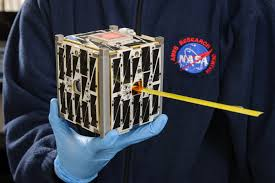
\includegraphics[scale=0.5]{figures/cubesat.jpg}
\caption{Referência de Tamanho de um Cubesat}
\label{figura_cubesat}
\end{center}
\end{figure}

Um dos novos desafios de desenvolvimento para \textit{Cubesats} é a limitação no orçamento, a qual torna necessária a realização de modelagens e simulações antes do desenvolvimento do produto, de forma a reduzir os custos. Outro desafio é a limitação na área disponível para captação e armazenamento de energia devido ao tamanho dos satélites\cite{Kalman2011}. Tendo em vista esta limitação no aspecto energético, é necessário projetar o sistema cuidadosamente de forma que a energia fornecida pelos painéis solares e armazenadas nas baterias seja suficiente para alimentar as cargas do sistema.

Os \textit{Cubesats} são, em geral, compostos por um Computador de Bordo, responsável por gerenciar os dados do satélite, um \gls{eps}, responsável por captar, armazenar e distribuir energia para os outros módulos, um Sistema de Comunicação, capaz de enviar e receber dados e comandos para a Terra e, por fim, os \textit{payloads}, que são a carga útil do sistema, ou seja, realizam a função principal do satélite.

Os \gls{eps} usam como principal entrada de energia painéis solares, que são a fonte mais abundante no espaço. Outra maneira de se captar energia é através de termogeradores. Para armazenar a energia são usadas geralmente bateris Li-Ion, porém alguns projetos utilizam supercapacitores ou baterias de composição diferente.

Neste trabalho será apresentado o \gls{eps} do \textit{Cubesat} FloripaSat, atualmente em desenvolvimento na UFSC, com foco no gerenciamento da energia, desde a entrada até o consumo dos outros módulos. Este \gls{eps} tem como entrada de energia painéis solares, que são conectados através de um conversor \textit{boost} a duas baterias Li-Ion conectadas em série. Um algortimo \gls{mppt} é utilizado para operar os paineis com máxima eficiência. O sistema distribui a energia para os outros módulos do satélite (computador de bordo, sistema de comunicação e \textit{payloads}) em diferentes tensões através de conversores CC-CC integrados. Será realizada a modelagem do sistema, simulações e, por fim, testes com o sistema real, de forma que será possível validar a simulação para trabalhos futuros assim como verificar se o sistema projetado está de acordo com o necessário.

\section{Objetivos}

Esta seção apresenta o objetivo geral e os objetivos específicos deste trabalho.

\subsection{Geral}

Modelar, simular e testar o funcionamento do módulo de energia do nanossatélite Floripa-Sat.

\subsection{Específicos}
\begin{itemize}
\item Modelar os painéis solares
\item Modelar o conversor boost da entrada
\item Modelar o consumo do \textit{Cubesat}
\item Simular o sistema completo
\item Realizar testes com o sistema real
\item Comparar os resultados reais com os simulados
\end{itemize}

\section{Organização do trabalho}

O capítulo \ref{secao:painel solar} apresenta brevemente o funcionamento dos paineis solares, um circuito equivalente com componentes representando a conversão de energia solar em energia elétrica e as perdas, um modelo do painel real a ser utilizado no trabalho e por fim algoritmos para operação do painel com máxima eficiência.

No capítulo \ref{secao:conversores_cc_cc} são apresentadas duas maneiras de se utilizar conversores CC-CC no controle da operação de paineis solares e uma modelagem simplificada a ser utilizada na simulação do sistema.

O próximo passo é a modelagem das cargas do sistema (capítulo \ref{secao:modelagem_cargas}), para possibilitar a verificação do funcionamento do sistema na simulação. Para tal foram utilizadas informações fornecidas nos \textit{datasheets} dos principais componentes de cada módulo do satélite (comunicação, computador de bordo, sistema de energia e \textit{payloads}).

Nos capítulos \ref{secao:simulacao_sistema} e \ref{secao:teste_sistema}, respectivamente, são apresentados as simulações e testes realizados na bancada para verificar se o sistema projetado atende os requisitos de carga e também validar a simulação realizada em comparação com o sistema real.

Ao final do trabalho são apresentadas as conclusões sobre o que foi proposto e desenvolvido (capítulo \ref{secao:conclusoes}).


